\documentclass[12pt,fleqn]{article}\usepackage{../../common}
\begin{document}
Eğri Uydurma, Aradeğerleme (Interpolation) - 3

Spline Eğrileri

Diyelim ki elimizde 4 $x_i,y_i$ noktası var, ve bu noktalardan geçen,
hepsinden {\em kesinlikle} geçen, yaklaşıksal bir eğri oluşturmak
istiyoruz. Spline yöntemi her iki nokta arasını farklı bir küpsel (üçüncü
derece) polinom ile temsil etmektir. Tekrar dikkat: tüm noktaları temsile
edebilecek farklı polinomları toplamıyoruz, her aralıkta başka bir polinom
fonksiyonu parçasını devreye sokuyoruz. Parçalar niye küpsel olarak
seçildi? Çünkü küpsel bir eğri yeterince kavis sağlayabilir ve aynı zamanda
çok fazla inişli çıkışlı, sivri değildir, yeterince pürüzsüz bir eğrinin
ortaya çıkmasını sağlar.

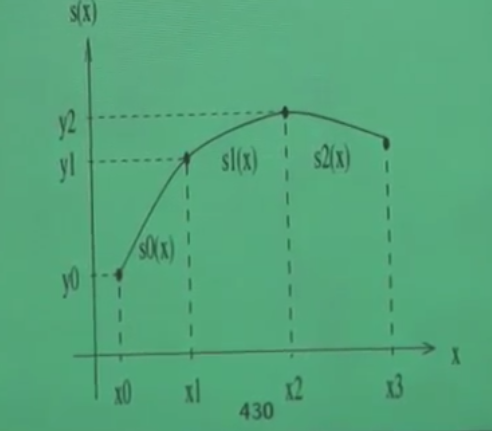
\includegraphics[height=4cm]{spline1.png}

Her $i=0,..,n+1$ için 

$$ p(x) = p_i(x) = a_i + b_i(x-x_i) + c_i(x-x_i)^2 + d_i(x-x_i)^3
\mlabel{1}
$$

kullanalım. Noktalar $x_i$ olarak gösteriliyor, ve her noktada aktif olan
bir $p_i$ spline olacak, o noktadan bir sonrakine kadar eğriyi bu $p_i$
tanımlayacak. Noktaların sayısını $n$ yerine $n+1$ olarak aldık böylece $n$
eğri parçası ile çalışmamız mümkün olacak. Her spline bir küpsel polinom ise
niye bu küpsel polinomu en basit şekliyle

$$ p(x) = a_i + b_ix + c_ix^2 + d_ix^3 $$

olarak tanımlamadık? Çünkü iki üstteki form ile çalışmak daha
rahat. Mesela, eğer $x$ için $x_i$ değrini verirsek, ki bu $x_1$ ya da
$x_2$ olabilirdi, o zaman parantez içinde $x_i - x_i$ sayesinde tüm 
terimler sıfır oluyor, geriye sadece $a_i$ kalıyor. 

Parçaların uçlarının birbirini tutması, ve tüm şeklin sürekli, akışkan bir
şekilde gözükmesi için ise birkaç koşulu bizim tanımlamamız, ve zorlamamız
gerekli. Önce en basit olanı: bir önceki parça ile bir sonraki parça
orta nokta üzerinde aynı değere sahip olmalı. $i=1,..,n+1$ için

$$ p_i (x_{i+1}) = p_{i+1}(x_{i+1}) $$

Bir diğer basit gereklilik, her $x_i$'ye tekabül eden spline fonksiyonun
elimizdeki $y_i$ değerini vermesi,

$$ p_i(x_i) = y_i $$

``Tüm noktalardan kesinlikle geçmeli'' demiştik. Son parça bir istisna
oluşturuyor, bu son parçanın fonksiyonu hem son noktayı, hem de ondan bir
önceki nokta için kullanılmalı, bir önceden en sona kadar aynı fonksiyon
üzerindeyiz. 

$$ p_{n}(x_n) = y_{n+1} $$

Sistemi daha detaylı olarak görmek gerekirse, tüm denklemleri yazalım,

$$ p_1(x)  = a_1 + b_1(x-x_1) + c_1(x-x_1)^2 + d_1(x-x_1)^3$$

$$ p_2(x)  = a_2 + b_2(x-x_2) + c_2(x-x_2)^2 + d_1(x-x_2)^3$$

$$ \vdots $$

$$ p_n(x)  = a_n + b_n(x-x_n) + c_n(x-x_n)^2 + d_3(x-x_n)^3$$

Üç noktalı şöyle bir grafik düşünelim,

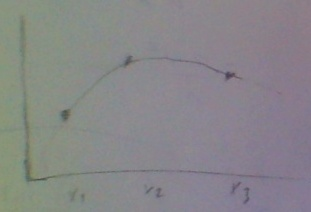
\includegraphics[height=4cm]{spline2.png}

Üstte bahsettiğimiz gibi, $p_1(x_1) = a_1 = y_1$ olacak, ve tüm indisler
için bu geçerli. Ayrıca $x_2$ noktasında bir önceki parça ve sonraki parça
aynı değere sahip olmalı demiştik, yani mesela $p_1$'in sonunda (üstteki
ilk parça) $x_2$ noktası vardır, ve aynı noktada $p_2$ başlayacaktır, o
noktada $$ p_1(x_2) = a_1 + b_1h_1 + c_1h_1^2 + d_1h_1^3  $$

ve bu denklem $p_2(x_2) = a_2 = y_2$'ye eşit. Bir de, daha önce gördük, $a_1 =
y_1$ ise, o zaman 

$$ y_2 = p_1(x_2) = y_1 + b_1h_1 + c_1h_1^2 + d_1h_1^3 $$

haline gelir. Hepsini birarada yazıyoruz ($y$'yi sağ tarafa aldık)

$$ y_1 + b_1h_1 + c_1h_1^2 + d_1h_1^3 = y_2 
\mlabel{2} 
$$

$$ y_2 + b_2h_2 + c_2h_2^2 + d_2h_2^3 = y_3 $$

$$ \vdots $$

$$ y_n + b_nh_n + c_nh_n^2 + d_nh_n^3 = y_n $$

ki $h_1 \equiv x_2 - x_1$, $h_2 \equiv x_3 - x_2$ olarak tanımladık,
$\equiv$ işareti ``tanımlamak (defined as)'' anlamına geliyor, $h$
harfi bir tür kısaltma olarak kullanıldı. Fakat kesintisizlik için
parçaların uçlarının bitişmesi yeterli değil. Mesela alttaki figürün de
uçları birleşiktir,

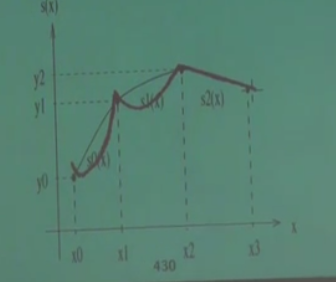
\includegraphics[height=4cm]{spline3.png}

Demek ki ek bazı şartlar lazım. Bu ek şart ``süreklilik'' olabilir. Mesela
alttaki örnek sürekli değildir.

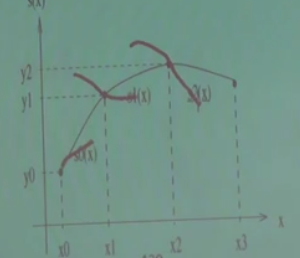
\includegraphics[height=4cm]{spline5.png}

Ya da daha iyisi, fonksiyonun her noktada ``türevi alınabilir'' olma
şartı. Mesela altta koyu yuvarlaklı gösterilen noktada fonksiyonun türevi
alınamaz.

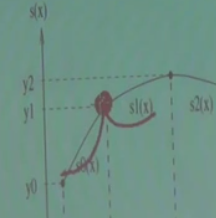
\includegraphics[height=4cm]{spline4.png}

O zaman şartı koyalım -- Fonksiyonun her noktasında, ikinci türev sürekli
alınabilmeli. Bu çok ağır / net bir şart aslında, ve hakikaten çok pürüzsüz
(smooth) fonksiyonların oluşmasına sebep oluyor. Şimdi bunun ne anlamına
biraz daha yakından bakalım. Biliyoruz ki futbol sahalarının etrafında koşu
alanı vardır. Bu alan şöyledir.

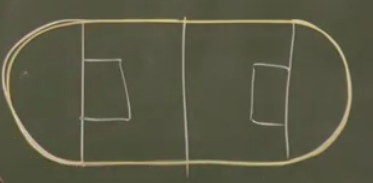
\includegraphics[height=4cm]{spline6.png}

Bu şekil iki ayrı figürün birleşimidir aslında, düz çizgiler ve iki tane
yarı çember. Üstteki düz çizgili kısım sonsuz kere türevi alınabilir bir
fonksiyondur. Değil mi? Düz çizgi sabit bir sayıdır, 1. türev sıfır, ikinci
türev yine sıfır, böyle gider. Peki yarı çember olan kısımlar? Aynı
şekilde. Peki her noktada durum böyle midir? Kritik noktalar ufak
yuvarlaklarla gösterilen yerler (altta)

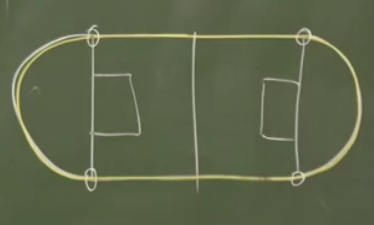
\includegraphics[height=4cm]{spline7.png}

Bu noktalarda kaç kere ``sürekli türevler'' alınabilir? Cevap, sadece bir
kere. Çünkü iki kere türev alınınca ne olacağına bakalım, düz kısımda
ikinci, üçüncü, vs. türev sıfır. Peki yarı çember? Onun ikinci türevi sıfır
olmayan sabit bir sayı. O zaman fonksiyonun tamamının (düz çizgi ve yarı
çemberin beraber) 2. türevini grafiklesek, şöyle bir şekil ortaya çıkardı,

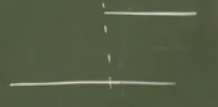
\includegraphics[height=4cm]{spline8.png}

ve bu grafikte görüyoruz ki bir zıplama var. Bu zıplama yüzünden süreklilik
(2. türevde) bozulmuş oldu. O zaman spline düzgün, pürüzsüz olsun istiyorsak, her noktada, yani
bağlantı noktalarında, sağdaki ve soldaki parçanın birinci ve ikinci
türevinin aynı olması şartını koyabiliriz, o zaman bu noktalarda
fonksiyonun tamamı iki kere sürekli türevi alınabilir hale
gelir. Parçaların kendisi üzerinde bu şartı tanımlamaya gerek yok, çünkü
orada polinom kullanacağımızı belirttik zaten, polinomlar sonsuz kere
sürekli türevi alınabilen objelerdir. 

Denklem sistemimize iki tane daha şart gerekiyor. Bu şartlar fonksiyonun
ilk noktada ve son noktada ikinci türevinin sıfır olması şartı
olabilir. Her hangi yöndeki bir çizgi $y = ax + b$'nin iki kere türevi
alınınca sıfır gelir, yani bu şart fonksiyonumuzun son noktalarda,
fonksiyonun ``aşağı yukarı aynı yönde'' olacak şekilde düz olarak devam
etmesi anlamına geliyor. Yaklaşıksal bağlamda fena bir şart değil. 

O zaman ana formüllerimize dönelim, ve mesela $p_1(x),p_2(x)$'in türevini
alalım,

$$ p_1'(x) = b_1 + 2c_1h_1 + 3d_1h_1^2 $$

$$ p_2'(x) = b_2 + 2c_2h_2 + 3d_2h_2^2 $$

$$ \vdots $$

Türevleri eşitleyelim $p_1'(x_2) = p_2'(x_2)$. 

$$ p_1'(x_2) = b_1 + 2c_1h_1 + 3d_1h_1^2 $$

$$  p_2'(x_2) = b_2 $$

Üstteki niye sadece $b_2$ oldu? Çünkü $x_i-x_i$ numarası onun için de
geçerli, geriye sadece $b_2$ kaldı. Hepsi bir arada

$$  b_1 + 2c_1h_1 + 3d_1h_1^2  = b_2 
\mlabel{3}$$

$$  b_2 + 2c_2h_2 + 3d_2h_2^2 = b_3 $$

$$ \vdots $$

$$  b_{n-1} + 2c_{n-1}h_{n-1} + 3d_{n-1}h_{n-1}^2 =  b_n $$

İkinci türevler için benzer bir durum var, bu sefer sol taraftan $b$'ler
yokoluyor, 

$$ 2c_1 + 6d_1h_1 = 2c_2 
\mlabel{4} $$

$$ 2c_2 + 6d_2h_2 = 2c_3 $$

$$ \vdots $$

$$ 2c_{n-1} + 6d_{n-1}h_{n-1} = 2c_n $$

İlk ve son ikinci türevi sıfıra eşitlemeyi unutmayalım. Son türev

$$ 2c_n + 6d_nh_n = 2c_{n+1} = 0 $$

İlk türev

$$ p_1''(x_1) =  c_1 + 6d_1(x_1-x_1)  = c_1 = 0$$

$$ 6d_1(x_1-x_1) $$ sıfır olur

Denklem (4)'den başlayan bölümü tekrar düzenlersek, 

$$ d_1 = \frac{ c_2 - c_1}{3h_1} 
\mlabel{5} $$

$$ d_2 = \frac{ c_3 - c_2}{3h_2} $$

$$ \vdots $$

$$ d_n = \frac{ c_{n+1} - c_n}{3h_n} $$

Üstteki denklemleri (2) ve (3)'e geri koyarsak,

$$ b_1 + \frac{ c_2 + 2c_1}{3}h_1 = s_1 
\mlabel{7} $$

$$ b_2 + \frac{ c_3 + 2c_2}{3}h_1 = s_2 $$

$$ \vdots $$

$$ b_n + \frac{ c_{n+1} + 2c_n}{3}h_n = s_n $$

ki $s_1 \equiv \frac{y_2 - y_1}{h_1}, s_2 \equiv \frac{y_3 - y_2}{h_2}$. 

(3) ifadesini alıp tekrar düzenlersek, 

$$  2c_1h_1 + 3d_1h_1^2  = b_2 - b_1$$

$3d_1h_1$ için başka bir ifade kullanabiliriz, eğer (5)'i tekrar
düzenlersek,

$$ 3h_1d_1 = c_2 - c_1$$

ve iki üstteki formüle koyarsak

$$  2c_1h_1 + (c_2 - c_1)h_1  = b_2 - b_1$$

$$  2c_1h_1 + c_2h_1 - c_1h_1  = b_2 - b_1$$

$$  c_1h_1 + c_2h_1  = b_2 - b_1$$

$$  (c_1 + c_2) h_1  = b_2 - b_1$$

Bu ifade tüm $i$ noktaları için geçerli, hepsi bir arada

$$  (c_1 + c_2) h_1  = b_2 - b_1 
\mlabel{6}$$

$$  (c_2 + c_3) h_2  = b_3 - b_2$$

$$ \vdots $$

$$  (c_{n-1} + c_n) h_{n-1}  = b_n - b_{n-1}$$

(7)'deki ardı ardına gelen denklemleri birbirinden çıkartıp sonucu 3 ile
çarparsak, 

$$ c_1h_1 + 2c_2(h_1 + h_2) + c_3h_2 = 3(s_2 - s_1) $$

$$ c_2h_2 + 2c_3(h_2 + h_3) + c_4h_3 = 3(s_3 - s_2) $$

$$ \vdots $$

$$ c_{n-1}h_{n-1} + 2c_n(h_{n-1} + h_{n}) + c_{n+1}h_n = 3(s_n - s_{n-1}) $$

Bu formüller birarada düşünülürse, bilinmeyenleri $c_2,c_3,..,c_n$ olan
normal (ordinary) $n-1$ tane lineer denklemdirler, ve bir matris çarpımı
olarak düşünülebilirler. 

$c_1h_1$ matris formunda yok çünkü $c_1=0$. 

$$ 
\left[\begin{array}{cccccc}
2(h_1+h_2) & h_2 & 0 & 0 & ... & 0 \\
h_2 & 2(h_2+h_3) & h_3 & 0 & .. & 0  \\
0 & h_3 & 2(h_3+h_4) & h_4 & .. & 0 \\
0 & 0 & h_4 & 2(h_4+h_5) & ... & 0 \\
\vdots & \vdots & \vdots & \vdots & \ddots & \vdots  \\
0 & 0 & .. & 0 & h_{n-1} & 2(h_{n-1}+h_n) 
\end{array}\right]
\left[\begin{array}{r}
c_2 \\ c_3 \\ \vdots \\ c_n
\end{array}\right]
 $$

Bu denklem sağ tarafta suna eşit 

$$ 
\left[\begin{array}{r}
3(s_2 - s_1) \\
3(s_3 - s_2) \\
3(s_4 - s_3) \\
\vdots \\
3(s_n - s_{n-1}) 
\end{array}\right]
 $$

 Bir üçgen köşegen (tridiagonal) matris iki tane ikili köşegen (bidiagonal)
 matrisin çarpımına eşittir. LU çarpanlarına ayırma işlemi de, bkz [5], bize
 bu matrisleri sağlayacaktır.

$$ Ax = b $$

şu hale gelir

$$ LUx = b $$

Şimdi eğer $Ux = y$ kabul edersek, yani yeni bir değişkeni dahil edersek,
$L$'i bulduktan sonra

$$ Ly = b $$

kabul edebiliriz, ve bu formülü de $y$ için çözmek çok kolaydır. Sonra
çözülen $y$'yi alıp geriye sokma (backsubstitution) ile $x$'i buluruz, yani 

$$ Ux = y $$ 

denklemini çözeriz. 

\begin{minted}[fontsize=\footnotesize]{python}
import scipy.linalg as lin

a = np.array( [[3.,-3.,0,0],
               [-3.,8.,-2.,0],
               [0,1.,2.,4.],
               [0,0,-2.,6.]])

p,l,u = lin.lu(a)

Ly = np.array([[7.,8.,2.,-3.]])

y = lin.solve(l,Ly.T)

x = lin.solve(u,y)
print x
\end{minted}

\begin{verbatim}
[[ 5.44047619]
 [ 3.10714286]
 [ 0.26785714]
 [-0.41071429]]
\end{verbatim}

Spline yöntemine dönersek, elimizdeki veri ve kod şöyle olsun

\begin{minted}[fontsize=\footnotesize]{python}
import scipy.linalg as lin

xx = np.array([4.,9.,12.,16.,22.])

yy = np.array([157.,41.,145.,92.,7.])

h = np.diff(xx)

dy = np.diff(yy)

s = dy / h

ds = np.diff(s)

s3 = 3 * ds

a = np.array([[ 2*(h[0]+h[1]), h[1], 0],
              [ h[1], 2*(h[1]+h[2]), h[2]],
              [ 0, h[2], 2*(h[2]+h[3])]])

p,l,u = lin.lu(a)

y = lin.solve(l,s3.T)

c = lin.solve(u,y)
print c
\end{minted}

\begin{verbatim}
[ 13.45756677 -13.90702275   2.64390455]
\end{verbatim}

$c$'ler bulunduktan sonra $h$'lerle beraber kullanılarak $d$'ler bulunur,
vs, ve tüm spline parçalarının katsayıları ortaya çıkartılır.

Kodlar

Bazı kodlar altta bulunabilir. İlk önce SciPy ile B-spline, ilmikleri biz
dışarıdan tanımladık, 

\begin{minted}[fontsize=\footnotesize]{python}
from scipy.interpolate import splev, splrep
x = np.linspace(0, 10, 10)
y = np.sin(x)
tck = splrep(x, y, t=[4,8]) # ilmikler t icinde
x2 = np.linspace(0, 10, 200)
y2 = splev(x2, tck)
plt.plot(x, y, 'o', x2, y2)
plt.savefig('compscieng_1_21_05.png')
\end{minted}

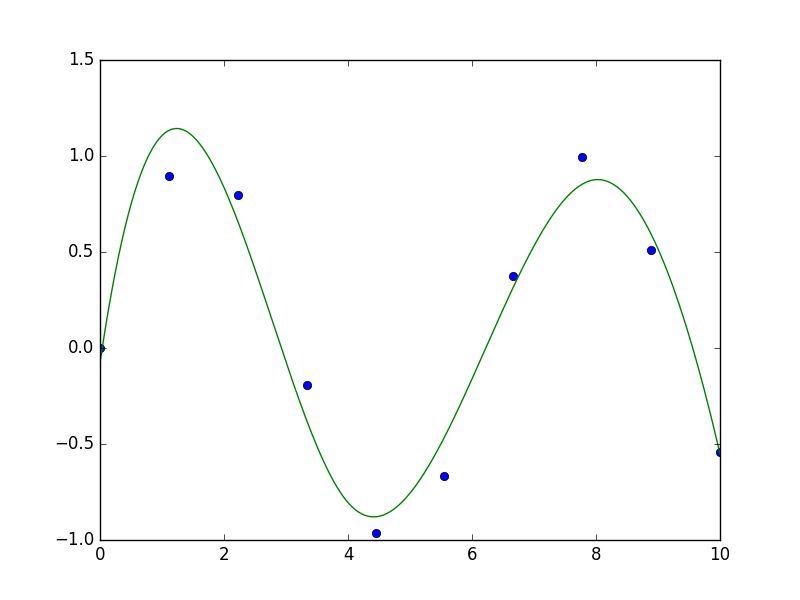
\includegraphics[width=20em]{compscieng_1_21_05.png}

Alttaki kodlar tüm eğrinin verideki her noktayı ilmik olarak görmesi
gerektiğine göre yazılmıştır, yani her veri noktası aynı zamanda bir
ilmiktir.

\inputminted[fontsize=\footnotesize]{python}{Spline.py}

\begin{minted}[fontsize=\footnotesize]{python}
import Spline
x = lambda n: np.linspace(-1,1,n)
f = lambda x: np.cos(np.sin(np.pi*x))
n = 5
E=200
data = zip(x(n),f(x(n)))
splines,xn = Spline.Splines(data)
X,Y = Spline.splinesToPlot(splines,xn,E)
plt.plot(X,Y,'r--')
plt.plot(x(300),f(x(300)),'k')
plt.savefig('compscieng_1_21_04.png')
\end{minted}

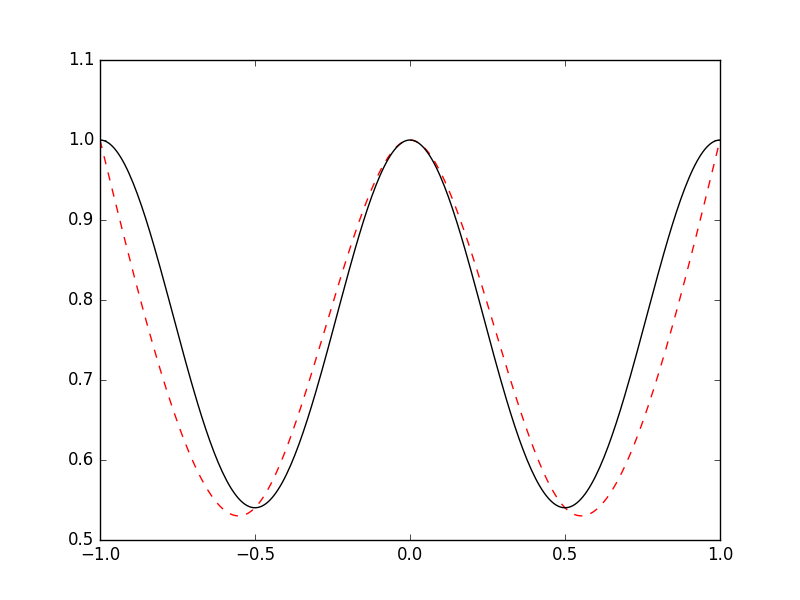
\includegraphics[height=6cm]{compscieng_1_21_04.png}

Bir diğer örnek

\inputminted[fontsize=\footnotesize]{python}{cubicSpline.py}

\begin{minted}[fontsize=\footnotesize]{python}
import pandas as pd, cubicSpline
df = pd.read_csv('in.csv')
res = cubicSpline.curvatures(np.array(df.x), np.array(df.y))
print res
\end{minted}

\begin{verbatim}
[ 0.         -2.27960615  0.5983445  -2.14369027 -0.5421918  -0.9485407
  4.83823742  1.40244849 -0.82589911 -1.3439826   2.52298704  0.        ]
\end{verbatim}

Kaynaklar

[1] Vrbik, {\em MATH 2P20 NUMERICAL ANALYSIS I Lecture Notes}, \url{http://spartan.ac.brocku.ca/~jvrbik/MATH2P20/notes.pdf}

[2] Ertel, {\em Advanced Mathematics for Engineers Lecture No. 14}, \url{http://www.youtube.com/watch?v=3rHBCglD1LQ}

[3] Ertel, {\em Advanced Mathematics for Engineers Lecture No. 15}, \url{http://www.youtube.com/watch?v=nA0YpqraP9A}

[4] Recktenwald, {\em Numerical Methods with MATLAB Implementations and Applications}

[5] Bayramlı, Lineer Cebir, {\em Ders 4}



\end{document}
